% Created 2016-05-27 Fri 18:15
\documentclass[9pt,b5paper]{article}
\usepackage{fontspec}
\setmainfont{STSong}
\usepackage{graphicx}
\usepackage{xcolor}
\usepackage{xeCJK}
\setCJKmainfont{STSong}
\usepackage{longtable}
\usepackage{float}
\usepackage{textcomp}
\usepackage{geometry}
\geometry{left=0cm,right=0cm,top=0cm,bottom=0cm}
\usepackage{multirow}
\usepackage{multicol}
\usepackage{listings}
\usepackage{algorithm}
\usepackage{algorithmic}
\usepackage{latexsym}
\usepackage{natbib}
\usepackage[xetex,colorlinks=true,CJKbookmarks=true,linkcolor=blue,urlcolor=blue,menucolor=blue]{hyperref}


\lstset{language=c++,numbers=left,numberstyle=\tiny,basicstyle=\ttfamily\small,tabsize=4,frame=none,escapeinside=``,extendedchars=false,keywordstyle=\color{blue!70},commentstyle=\color{red!55!green!55!blue!55!},rulesepcolor=\color{red!20!green!20!blue!20!}}
\author{deepwaterooo}
\date{\today}
\title{Programming Language Theory -- Summer 2016}
\hypersetup{
  pdfkeywords={},
  pdfsubject={},
  pdfcreator={Emacs 24.5.1 (Org mode 8.2.7c)}}
\begin{document}

\maketitle
\tableofcontents


\section{Introduction}
\label{sec-1}
\begin{itemize}
\item Zombies are coming\textasciitilde{}
\item Todos: 
\begin{itemize}
\item With struct help could have more fun dancing with more zombies, but need try hard to figure out how to dance with time changes (has not really got ideas today), or need to move according to keytype inputs triggers.
\item Sub obj\% for cubes, and spheres if I need and want to implement any sphere for head, or eyes.
\item My team buddy's spiderman I will try to figure out how to Texture or draw as the dancing stage.
\end{itemize}
\item A current rotatable zombie and my team buddy's spiderman are looking like:
\end{itemize}

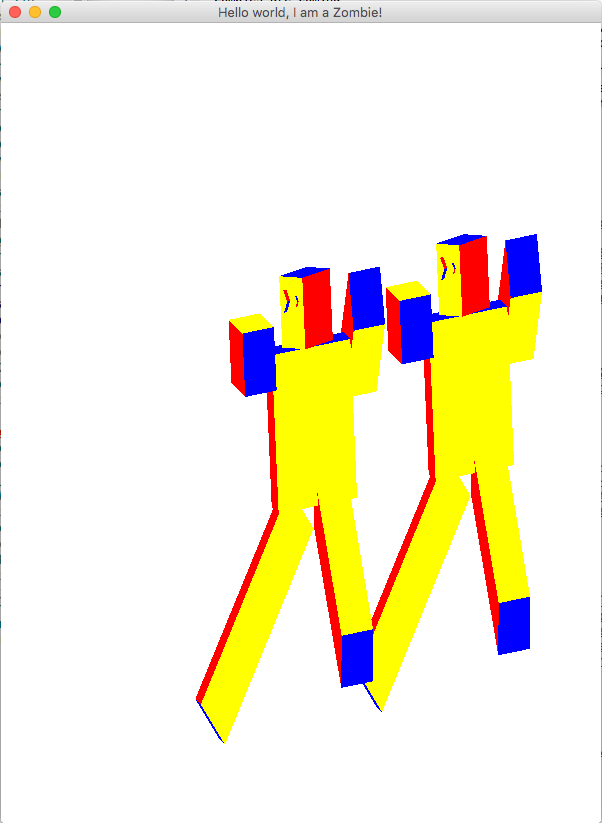
\includegraphics[width=.9\linewidth]{./pic/Screen_Shot_2016-05-27_at_6_04_21_PM.png}

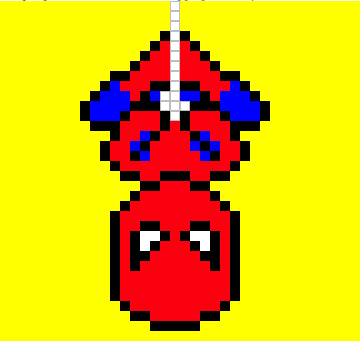
\includegraphics[width=.9\linewidth]{./pic/Screen_Shot_2016-05-27_at_6_08_17_PM.png}

\section{References}
\label{sec-2}
\subsection{opengl sgl}
\label{sec-2-1}
\begin{itemize}
\item rect hello world \url{https://lists.racket-lang.org/users/archive/2010-October/042474.html}
\item cube base: \url{https://gist.github.com/tonyg/5425736}
\item Texture Atlases \url{http://jeapostrophe.github.io/2013-05-06-texture--post.html}
\item Planet Cute \url{http://docs.racket-lang.org/teachpack/2htdpPlanet_Cute_Images.html}
\item Texture \url{https://www.mail-archive.com/racket-users@googlegroups.com/msg03203.html}
\item \url{http://lists.racket-lang.org/users/archive/2010-November/043118.html}
\item sgl \url{https://github.com/racket/sgl}
\item cube \url{https://rosettacode.org/wiki/Draw_a_cuboid#Racket}
\item pict3d \url{https://github.com/ntoronto/pict3d}
\item pict3d \url{https://docs.racket-lang.org/pict3d/index.html}
\item buffering \url{https://lists.racket-lang.org/users/archive/2015-March/066355.html}
\item c++ racket ex \url{http://home.adelphi.edu/sbloch/class/archive/333/fall2013/examples/pentagon/}
\item \url{https://rosettacode.org/wiki/OpenGL#Racket}
\item 原理: \url{http://cuiqingcai.com/1867.html}
\item \url{http://cuiqingcai.com/1867.html}
\item 2d \url{http://cuiqingcai.com/1597.html}
\item tech cube \url{http://wiki.jikexueyuan.com/project/opengl-es-basics/3d-images.html}
\item colorful \url{http://cs317y982s961535.blogspot.com/2010/04/2-3d.html}
\item \url{http://www.d3dweb.com/Documents/201202/15-15182458704.html}
\item define-struct \url{http://lists.racket-lang.org/users/archive/2008-July/026133.html}
\item class ex \url{https://learnxinyminutes.com/docs/racket/}
\item gui \url{https://docs.racket-lang.org/pict3d/rendering.html}
\end{itemize}
\subsection{Animation}
\label{sec-2-2}
\begin{itemize}
\item 3d programming: \url{http://cs317y982s950831.blogspot.com/}
\item ruby \url{https://www.youtube.com/watch?v=Iq5YbRDYVE4}
\item ex \url{https://www.ntu.edu.sg/home/ehchua/programming/opengl/CG_Examples.html}
\item sphere Texture \url{http://www.angelfire.com/linux/nexusone/projects.html}
\item sphere \url{https://www.opengl.org/discussion_boards/showthread.php/137753-Texture-map-on-a-gluSphere}
\item s trs \url{https://www.opengl.org/discussion_boards/showthread.php/163561-How-to-posistion-a-gluSphere}
\item emacs lambda \url{http://ergoemacs.org/emacs/emacs_pretty_lambda.html}
\item 
\item 
\end{itemize}

\section{OOP}
\label{sec-3}
\begin{itemize}
\item oop \url{https://docs.racket-lang.org/guide/classes.html}
\item creating classes \url{https://docs.racket-lang.org/reference/createclass.html}
\item 
\item 
\end{itemize}

\subsection{robot dance}
\label{sec-3-1}
\begin{itemize}
\item \url{https://www.youtube.com/watch?v=lacAgc7rv1o}
\item \url{https://www.youtube.com/watch?v=AoCXPicEa8o}
\item \url{https://www.youtube.com/watch?v=wQ4KXoFHwL4}
\item 
\item 
\end{itemize}

\subsection{other}
\label{sec-3-2}
\begin{itemize}
\item framework \url{https://github.com/NetEase/lively-logic}
\item \url{https://www.youtube.com/watch?v=SCh0zmP6R5A}
\item \url{https://www.youtube.com/watch?v=ayqhX9UA6FY}
\item \url{http://racket.tchen.me/practical-racket.html}
\item 图形:\url{https://www.zhihu.com/question/20789155}
\item threads \url{http://www.ithao123.cn/content-4141200.html}
\item \url{http://docs.racket-lang.org/guide/classes.html}
\item \url{https://docs.racket-lang.org/quick/}
\item \url{http://docs.racket-lang.org/draw/index.html}
\item 
\item 
\end{itemize}
% Emacs 24.5.1 (Org mode 8.2.7c)
\end{document}